% Requires in the preamble: \usepackage{tabularx} and \usepackage{float}
% Add the two references at the bottom of this file to your .bib file

\section{SusAF analysis}\label{sec:susaf}
\label{sec:susaf}

To look at how sustainable our TO-BE solution is, we have used the Sustainability Awareness Framework (SusAF) \parencite{duboc2020}, as presented in the lectures by John Krogstie. SusAF looks at the effects of a system in five dimensions: social, individual, environmental, economic and technical. Each effect is also placed on one of three levels \parencite{becker2016}:

\begin{itemize}
    \item \textbf{Immediate:} effects that come directly from using the system.
    \item \textbf{Enabling:} effects that come from using the system over time.
    \item \textbf{Structural:} long-term changes in the organisation or in society.
\end{itemize}

We have done the analysis for the TO-BE main model and for each of the three cases. For each of them, we have made a table with the effects, and a diagram that shows which dimension and level each effect belongs to and how the effects affect each other. The ID of an effect shows its dimension and level. For example, II1 is the first \textit{Individual} effect on the \textit{Immediate} level, and ENS1 is the first \textit{Environmental} effect on the \textit{Structural} level (S = Social, I = Individual, EN = Environmental, EC = Economic, T = Technical). We have also marked the IDs in the BPMN models, so that it is easy to see where in the process each effect comes from. Since the solution has not been implemented yet, the effects are our own predictions, and they should be checked again during the pilot described in the implementation plan.

\subsection{Main model}
\label{subsec:susaf-main}

Here we look at the TO-BE main model (Figure~\ref{fig:main_to-be}) as a whole, where one shared GenAI service is used in all three processes. This shows the effects of the solution as a whole, and not just of one case.

\begin{figure}[H]
    \centering
    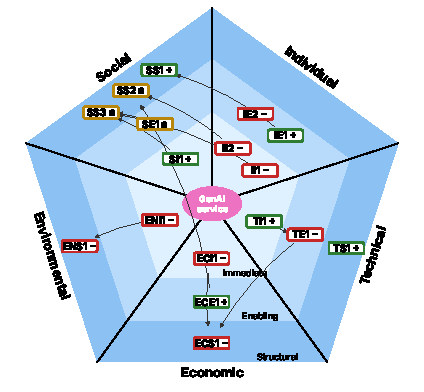
\includegraphics[width=0.6\textwidth]{Images/susaf/susad_main.pdf}
    \caption{Sustainability analysis diagram for Main model. Green: positive effect, red: negative effect, yellow: both. Arrows show that one effect leads to another.}
    \label{fig:susad-main}
\end{figure}

% Where to place each ID as an annotation in the BPMN models:
% TI1   -> GenAI service lane
% II1   -> GenAI service lane
% ENI1  -> GenAI service lane
% ECI1  -> GenAI service lane
% II2   -> Review and approve tasks (Teaching Staff, Study advisor)
% SI1   -> Review and approve tasks
% IE1   -> Student pool
% ECE1  -> Teaching Staff lane
% TE1   -> GenAI service lane
% IE2   -> Student pool
% SE1   -> Whole process
% SS1   -> Student pool
% SS2   -> Teaching Staff, Study advisor
% ECS1  -> GenAI service lane
% TS1   -> Whole process
% SS3   -> Whole process
% ENS1  -> GenAI service lane
\begin{table}[H]
    \centering
    \small
    \begin{tabularx}{\textwidth}{|l|X|l|l|c|}
        \hline
        \textbf{ID} & \textbf{Impact} & \textbf{Level} & \textbf{Affects} & \textbf{+/--} \\ \hline
        TI1 & One shared GenAI service & Immediate & TE1 & $+$ \\ \hline
        II1 & Personal data in AI service & Immediate & SS3 & $-$ \\ \hline
        ENI1 & Higher energy use & Immediate & ENS1 & $-$ \\ \hline
        ECI1 & Licence and operating costs & Immediate & ECS1 & $-$ \\ \hline
        II2 & New review tasks for staff & Immediate & SS2 & $-$ \\ \hline
        SI1 & Humans approve AI output & Immediate & SS3 & $+$ \\ \hline
        IE1 & More personal support & Enabling & SS1 & $+$ \\ \hline
        ECE1 & Staff time freed & Enabling & SS2 & $+$ \\ \hline
        TE1 & Single point of failure & Enabling & ECS1 & $-$ \\ \hline
        IE2 & Over-reliance on AI & Enabling & -- & $-$ \\ \hline
        SE1 & Need for AI literacy & Enabling & SS3 & $\pm$ \\ \hline
        SS1 & More equal access to support & Structural & -- & $+$ \\ \hline
        SS2 & Changed roles for staff & Structural & -- & $\pm$ \\ \hline
        ECS1 & Dependency on AI vendor & Structural & -- & $-$ \\ \hline
        TS1 & Data for improving curriculum & Structural & -- & $+$ \\ \hline
        SS3 & Trust in digital teaching & Structural & -- & $\pm$ \\ \hline
        ENS1 & Larger IT carbon footprint & Structural & -- & $-$ \\ \hline
    \end{tabularx}
    \caption{SusAF analysis of Main model}
    \label{tab:susaf-main}
\end{table}

\textbf{Positive effects:} The biggest positive effects are for the students and the staff. Students get more personal support during the whole semester (IE1), and over time this can give more equal access to support, since it no longer depends on who asks for help or which TA you get (SS1). Since a lot of routine work is automated, the staff get more time for teaching and guidance (ECE1). Using one shared service for all three processes (TI1) is also simpler than having three separate tools, and the data from the service could later be used to improve courses and study programmes (TS1). That all AI output is approved by a person before it reaches the student (SI1) is important for trust.

\textbf{Negative effects:} Most of the negative effects come from the GenAI service itself. Personal data from recordings, submissions and FS is processed by an external service (II1), the service uses energy (ENI1), and NTNU has to pay for licences and for running it (ECI1). Because all three processes use the same service, it also becomes a single point of failure (TE1). In the long run, this can make NTNU dependent on one vendor (ECS1) and increase the university's carbon footprint (ENS1). The staff also get new review tasks (II2), and there is a risk that students rely too much on the AI (IE2).

\textbf{Effects that can go both ways:} Some of the effects can go both ways. Students and staff need to learn how GenAI works and where it fails (SE1), which takes time but also gives them useful skills. The new roles for the staff (SS2) can mean less routine work, but also that they lose parts of the job they find meaningful. In the end, trust in digital teaching (SS3) depends on how well NTNU handles the risks above, especially personal data and errors in the AI output.

\subsection{Case 1}
\label{subsec:susaf-case1}

For Case 1, we looked at the effects of letting a GenAI service make a transcript, a topic index and study material from each lecture recording (Figure~\ref{fig:case1-tobe}).

\begin{figure}[H]
    \centering
    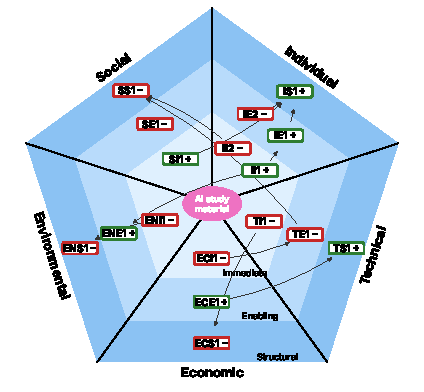
\includegraphics[width=0.6\textwidth]{Images/susaf/susad_case1.pdf}
    \caption{Sustainability analysis diagram for Case 1. Green: positive effect, red: negative effect, yellow: both. Arrows show that one effect leads to another.}
    \label{fig:susad-case1}
\end{figure}

% Where to place each ID as an annotation in the BPMN models:
% II1   -> Search topic index and transcript (b)
% SI1   -> Transcribe recording (a)
% II2   -> Transcribe recording (a)
% ENI1  -> Subprocess (a)
% ECI1  -> Review and approve AI-generated material (main)
% TI1   -> GenAI service lane
% ENE1  -> Jump to timestamp (b)
% IE1   -> Subprocess (b)
% IE2   -> Read summary and key points (b)
% SE1   -> Attend lectures (main)
% TE1   -> Review and approve AI-generated material (main)
% ECE1  -> Subprocess (a)
% IS1   -> Subprocess (b)
% TS1   -> Panopto database
% SS1   -> Whole process
% ECS1  -> GenAI service lane
% ENS1  -> GenAI service lane
\begin{table}[H]
    \centering
    \small
    \begin{tabularx}{\textwidth}{|l|X|l|l|c|}
        \hline
        \textbf{ID} & \textbf{Impact} & \textbf{Level} & \textbf{Affects} & \textbf{+/--} \\ \hline
        II1 & Faster search for concepts & Immediate & IE1, ENE1 & $+$ \\ \hline
        SI1 & Accessible transcripts & Immediate & IS1 & $+$ \\ \hline
        II2 & Recordings processed by AI & Immediate & SS1 & $-$ \\ \hline
        ENI1 & Energy use per lecture & Immediate & ENS1 & $-$ \\ \hline
        ECI1 & Extra review work for staff & Immediate & TE1 & $-$ \\ \hline
        TI1 & New integration to maintain & Immediate & ECS1 & $-$ \\ \hline
        ENE1 & Less streaming of full videos & Enabling & -- & $+$ \\ \hline
        IE1 & Less time per lecture & Enabling & IS1 & $+$ \\ \hline
        IE2 & Passive use of summaries & Enabling & IS1 & $-$ \\ \hline
        SE1 & Fewer attend lectures & Enabling & -- & $-$ \\ \hline
        TE1 & Errors approved unread & Enabling & SS1 & $-$ \\ \hline
        ECE1 & Made once per lecture & Enabling & TS1 & $+$ \\ \hline
        IS1 & Better learning outcomes & Structural & -- & $+$ \\ \hline
        TS1 & Reusable lecture archive & Structural & -- & $+$ \\ \hline
        SS1 & Trust in lecture material & Structural & -- & $-$ \\ \hline
        ECS1 & Dependency on AI vendor & Structural & -- & $-$ \\ \hline
        ENS1 & Larger footprint at scale & Structural & -- & $-$ \\ \hline
    \end{tabularx}
    \caption{SusAF analysis of Case 1}
    \label{tab:susaf-case1}
\end{table}

\textbf{Positive effects:} Most of the positive effects are for the students. When they can search for a concept and jump straight to the right part of the video (II1), they spend less time on each lecture (IE1). In our walkthrough, one 90-minute lecture took about three hours to go through, so there is a lot of time to save. This time can instead be used on understanding the content, which can give better learning outcomes (IS1). The transcripts also make the lectures easier to follow for students with hearing impairments or another first language (SI1). Since the material is made once per lecture and not once per student (ECE1), and students only watch the parts they need (ENE1), the solution also uses fewer resources overall. Over time, the recordings and the material can be reused as a searchable archive (TS1).

\textbf{Negative effects:} The recordings contain the voice and image of both lecturers and students, and these are now processed by an external AI service (II2). The processing also uses energy for every lecture (ENI1), which adds up when all recorded lectures are included (ENS1). The teaching staff get extra work, since they have to review the material for every lecture (ECI1), and under time pressure they might approve it without reading it properly (TE1). Both of these can reduce trust in the lecture material (SS1). There is also a risk that students just read the summaries instead of engaging with the lecture (IE2), or that fewer students show up to the lectures (SE1). Finally, the service has to be integrated with Panopto and Canvas and maintained (TI1), which makes the courses dependent on the AI vendor (ECS1).

\textbf{What this means for our solution:} The analysis supports two choices we made in the TO-BE model. The review step makes sure that someone is responsible for the material, and the quiz questions and own comments keep the students active, so that the material does not just replace the lecture.

\subsection{Case 2}
\label{subsec:susaf-case2}

For Case 2, we looked at the effects of letting a GenAI service draft scores and feedback, which the TAs then review and approve (Figure~\ref{fig:case2tobe}).

\begin{figure}[H]
    \centering
    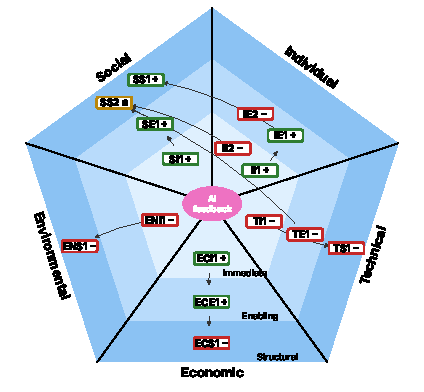
\includegraphics[width=0.6\textwidth]{Images/susaf/susad_case2.pdf}
    \caption{Sustainability analysis diagram for Case 2. Green: positive effect, red: negative effect, yellow: both. Arrows show that one effect leads to another.}
    \label{fig:susad-case2}
\end{figure}

% Where to place each ID as an annotation in the BPMN models:
% II1   -> Generate draft score and feedback (a)
% SI1   -> Generate draft score and feedback (a)
% II2   -> Retrieve submissions (a)
% ENI1  -> Generate draft score and feedback (a)
% ECI1  -> Review AI-drafted feedback (b)
% TI1   -> Retrieve solution and criteria (a)
% IE1   -> Read score and detailed feedback (main)
% TE1   -> Review AI-drafted feedback (b)
% IE2   -> Review AI-drafted feedback (b)
% ECE1  -> Subprocess (b)
% SE1   -> Whole process
% SS1   -> Student pool
% ECS1  -> Teaching Staff lane
% SS2   -> Whole process
% TS1   -> GenAI service lane
% ENS1  -> GenAI service lane
\begin{table}[H]
    \centering
    \small
    \begin{tabularx}{\textwidth}{|l|X|l|l|c|}
        \hline
        \textbf{ID} & \textbf{Impact} & \textbf{Level} & \textbf{Affects} & \textbf{+/--} \\ \hline
        II1 & Feedback for every student & Immediate & IE1 & $+$ \\ \hline
        SI1 & More consistent feedback & Immediate & SE1 & $+$ \\ \hline
        II2 & Submissions processed by AI & Immediate & SS2 & $-$ \\ \hline
        ENI1 & Energy use per submission & Immediate & ENS1 & $-$ \\ \hline
        ECI1 & Less TA time per submission & Immediate & ECE1 & $+$ \\ \hline
        TI1 & Requires explicit criteria & Immediate & TS1 & $-$ \\ \hline
        IE1 & Better writing and reasoning & Enabling & SS1 & $+$ \\ \hline
        TE1 & TA anchors on AI score & Enabling & SS2 & $-$ \\ \hline
        IE2 & Less meaningful TA work & Enabling & -- & $-$ \\ \hline
        ECE1 & Scales to larger cohorts & Enabling & ECS1 & $+$ \\ \hline
        SE1 & Fairer assessment & Enabling & SS2 & $+$ \\ \hline
        SS1 & Better learning outcomes & Structural & -- & $+$ \\ \hline
        ECS1 & Fewer TA positions & Structural & -- & $-$ \\ \hline
        SS2 & Trust in assessment & Structural & -- & $\pm$ \\ \hline
        TS1 & Need for system owner & Structural & -- & $-$ \\ \hline
        ENS1 & Larger footprint at scale & Structural & -- & $-$ \\ \hline
    \end{tabularx}
    \caption{SusAF analysis of Case 2}
    \label{tab:susaf-case2}
\end{table}

\textbf{Positive effects:} The most important positive effect is that every student gets detailed written feedback, and not just a score (II1). Over time, this can help the students improve their writing and reasoning (IE1), which is one of the goals in the case description (SS1). Since all drafts are based on the same criteria, the feedback also becomes more consistent (SI1), and the students are treated more equally no matter which TA they get (SE1). For the courses, the TA spends less time on each submission (ECI1), which makes it possible to give good feedback even in large courses (ECE1).

\textbf{Negative effects:} The same time saving can also lead to fewer TA positions (ECS1), which means that fewer students get the experience of being a TA. The TAs might also feel that the work is less meaningful when they mostly check AI drafts (IE2). A bigger problem for the assessment itself is that the TA might just accept the AI score instead of making their own assessment (TE1). Together with the fact that student submissions are processed by an AI service (II2), this can affect trust in the assessment (SS2). We have marked trust as both positive and negative, since more consistent feedback can also increase it. Generating feedback for every submission also uses energy (ENI1), which adds up across all courses (ENS1).

\textbf{What this means for our solution:} For the solution to work over time, the course coordinators need to write clear assessment criteria (TI1), and someone at NTNU has to own the system (TS1). The analysis also shows why it is important that the TA is still responsible for every score and comment.

\subsection{Case 3}
\label{subsec:susaf-case3}

For Case 3, we looked at the effects of the AI course recommender and the AI support for the study advisors (Figure~\ref{fig:case3-tobe}).

\begin{figure}[H]
    \centering
    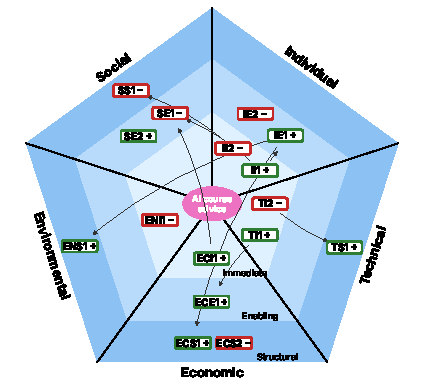
\includegraphics[width=0.6\textwidth]{Images/susaf/susad_case3.pdf}
    \caption{Sustainability analysis diagram for Case 3. Green: positive effect, red: negative effect, yellow: both. Arrows show that one effect leads to another.}
    \label{fig:susad-case3}
\end{figure}

% Where to place each ID as an annotation in the BPMN models:
% II1   -> Request AI course recommendation (a)
% II2   -> Retrieve student record (b)
% ENI1  -> Subprocess (b)
% ECI1  -> Get AI suggestions (c)
% TI1   -> Pre-check eligibility (b)
% TI2   -> Retrieve student record and course data (b)
% IE1   -> Compare recommended options (a)
% IE2   -> Compare recommended options (a)
% ECE1  -> Validate registration (main)
% SE1   -> Contact study advisor (a)
% SE2   -> Subprocess (a)
% ECS1  -> Whole process
% ECS2  -> Generate recommendations (b)
% SS1   -> Rank eligible courses (b)
% TS1   -> Course pages, Innsida
% ENS1  -> Whole process
\begin{table}[H]
    \centering
    \small
    \begin{tabularx}{\textwidth}{|l|X|l|l|c|}
        \hline
        \textbf{ID} & \textbf{Impact} & \textbf{Level} & \textbf{Affects} & \textbf{+/--} \\ \hline
        II1 & Personalised shortlist & Immediate & IE1, SE1 & $+$ \\ \hline
        II2 & Grades used by AI & Immediate & SS1 & $-$ \\ \hline
        ENI1 & Energy use per request & Immediate & -- & $-$ \\ \hline
        ECI1 & Faster advisor answers & Immediate & SE1 & $+$ \\ \hline
        TI1 & Eligibility checked by rules & Immediate & ECE1 & $+$ \\ \hline
        TI2 & Depends on course data & Immediate & TS1 & $-$ \\ \hline
        IE1 & Courses match goals & Enabling & ECS1, ENS1 & $+$ \\ \hline
        IE2 & Choice without reflection & Enabling & -- & $-$ \\ \hline
        ECE1 & Fewer rejected registrations & Enabling & -- & $+$ \\ \hline
        SE1 & Less contact with advisors & Enabling & -- & $-$ \\ \hline
        SE2 & Guidance for all students & Enabling & -- & $+$ \\ \hline
        ECS1 & Better match with job market & Structural & -- & $+$ \\ \hline
        ECS2 & Uneven course popularity & Structural & -- & $-$ \\ \hline
        SS1 & Bias reinforces inequality & Structural & -- & $-$ \\ \hline
        TS1 & Better course descriptions & Structural & -- & $+$ \\ \hline
        ENS1 & Fewer wrong choices & Structural & -- & $+$ \\ \hline
    \end{tabularx}
    \caption{SusAF analysis of Case 3}
    \label{tab:susaf-case3}
\end{table}

\textbf{Positive effects:} Most of the positive effects start with the student getting a personalised shortlist, instead of searching through all the courses on their own (II1). This makes it easier to choose courses that fit their interests and goals (IE1), which in the long run can give a better match with the job market (ECS1) and fewer wrong choices and extra semesters (ENS1). Because eligibility is checked by fixed rules and not by the language model (TI1), fewer registrations are rejected (ECE1). The study advisors also get help to answer faster (ECI1), and guidance is available to all students, not only the ones who contact an advisor (SE2). Since the recommender depends on good course data, NTNU will also have to keep the course pages up to date (TS1), which is useful for everyone.

\textbf{Negative effects:} The recommender uses grades and completed courses from FS (II2), which is personal data. There is a risk that recommendations based on grades steer some groups of students away from certain courses (SS1), and that courses that are often recommended get crowded while others lose students (ECS2). The students might also have less contact with advisors and other students when choosing courses (SE1), and some might just follow the recommendation without thinking it through (IE2). In addition, the recommender depends on integration with FS and up-to-date course data (TI2), and every request uses some energy (ENI1).

\textbf{What this means for our solution:} This shows that the recommendations need to be explained, and that the final choice has to stay with the student. We also think the recommender should be checked for bias during the pilot.


% ---------------- BibTeX entries ----------------
% @article{duboc2020,
%   author  = {Duboc, Leticia and Penzenstadler, Birgit and Porras, Jari and Akinli Kocak, Sedef and Betz, Stefanie and Chitchyan, Ruzanna and Leifler, Ola and Seyff, Norbert and Venters, Colin C.},
%   title   = {Requirements engineering for sustainability: an awareness framework for designing software systems for a better tomorrow},
%   journal = {Requirements Engineering},
%   volume  = {25}, number = {4}, pages = {469--492}, year = {2020},
%   doi     = {10.1007/s00766-020-00336-y}}
% @article{becker2016,
%   author  = {Becker, Christoph and Betz, Stefanie and Chitchyan, Ruzanna and Duboc, Leticia and Easterbrook, Steve M. and Penzenstadler, Birgit and Seyff, Norbert and Venters, Colin C.},
%   title   = {Requirements: The Key to Sustainability},
%   journal = {IEEE Software},
%   volume  = {33}, number = {1}, pages = {56--65}, year = {2016},
%   doi     = {10.1109/MS.2015.158}}
